\chapter{Design}
\label{sec:design}

This chapter will cover the process by which the code rewriting methodology employed by this thesis was designed. The chapter will start by defining the requirements and scope, followed by approaches that were considered and how the compiler-based approach was selected. This then leads into further design choices related to tools used to complete the deliverable. Finally, this chapter ends with the intended user flow for the rewrite tool and it's limitations.

\section{Requirements}

There is a basic set of requirements the methodology designed by this thesis must adhere to in order to be relatively realistic approach to the problem of code modernization. They are as follows:

\subsubsection{1. Code rewrites must not introduce, change, or remove side effects of rewritten operations}

This is a basic requirement that should be adhered to as much as possible. Approaches that increase the likelihood this rule is violated could make the tool difficult to use or even completely useless. Some important caveats related to this requirement are discussed in \ref{subsec:scope}.

\subsubsection{2. The approach should be automatic}

A common barrier to modernizing codebases is the combination of the complexity of the old code and the shear size of the codebase itself. Modern codebases can range from thousands of lines of code to millions. For example, the popular machine learning library TensorFlow is made up of about 4 million lines of code \cite{tf_loc}. Code written for modern vehicles is estimated to be about 100 million lines of code \cite{car_loc}. Even with a large team, manually modernizing even a moderately large codebase could be intractable on a reasonable timescale and could increase the likelihood other bugs associated with the rewrite are introduced. With this in mind, automating the modernization process as much as possible should be a defining requirement of the deliverable.

\subsubsection{3. Modifications must be reflected at the source level}

As discussed in Chapter \ref{sec:background}, there are domain specific development processes that require source to be reviewed before it can pass to the next step of the development pipeline. As a result, any approach that introduces checks for arithmetic operations must be able to show these changes at the source level for human review. Note that this technically implies the approach could introduce checks in code represented in some non-source (e.g. as an AST, IR, machine code, etc.) representation as long as the source could be reconstructed with the newly written checks.

\subsubsection{4. Users must be able to tailor how overflow detections are handled}

Handling integer overflows is completely context dependent and is thus impossible to write a one-size-fits-all handler. For example, it may be a very good idea to stop program execution when integer overflow is detected in some banking software, but not such a good idea in an engine controller. As such, the tool must allow the user to provide some rewrite code that acts as the error handler to tailor the system's response to any overflow detections.

\subsubsection{5. Users must be able to exempt lines from rewrites }

This is a usability requirement given some lines cannot be rewritten for some reason. This could be that there is an operation that is being rewritten that is out of scope of the tool, there is an error in the rewrite for a particular line, or some other unforeseen complication.

\subsubsection{6. Comments must be preserved}

Comments often contain important information for both humans or other processes in a development pipeline. Some approaches may remove comments since they operate using source stripped of any comments or on artifacts later in the compilation pipeline that don't contain source (and thus comments).

\section{Scope}
\label{subsec:scope}

With the requirements defined for the code modernization tool, this section will consider the scope of the rewrite tool. This includes the types of operations that will be rewritten, types of operands that will be considered, and the types of build systems this tool will focus on.

\subsection{Target Operations}

The new C23 checked arithmetic headers only include checks for addition, subtraction, and multiplication operations \cite{ckd_arith}. As mentioned in Chapter \ref{sec:background}, there are other operations and patterns that can trigger in integer overflow. Because of this, the rewrite tool will only be concerned with checked operations supported by C23 and their different forms. For addition, this includes the forms + (non-assignment operator), += (assignment operator), and ++ (unary operator). Furthermore, the tool will ignore any overflows due to other operations or casting errors not directly associated with these operations. The rational behind this is as long as the expression's type is the same in the AST before and after the rewrite, no casting errors can be introduced in the code. The downside is if there is a casting error higher up in the AST, the rewrite would preserve that error.

\subsection{Types and Other Language Features}

Again due to C23's checked arithmetic macros, arguments must be ``an integer type other than plain char, bool, a bit-precise integer type, or an enumeration type" \cite{ckd_arith}. This further limits the type of expressions that can be written with these macros, and thus limits the types of expressions the tool can support. In addition to this, a type that cannot be used is the ``bit-precise integer type". This is in reference to the \texttt{\_BitInt(n)} type also introduced in C23. This is a new integer type and thus not commonly in use especially by codebases written before the C23 standard was published. As a result, how the tool rewrites or does not rewrite expressions involving bit-precise integer types is considered out of scope for this project.

Macros and other expansion features \cite{macros} used by the preprocessor included in the C programming language could complicate a checked arithmetic rewriting tool. These include \texttt{\#includes}, \texttt{\#defines} and \texttt{\#/\#\#} directives, just to name a few. These features are used heavily in modern codebases, however in the context of this thesis it complicates the problem beyond what is needed to solve the core questions of this exploration. Furthermore, it is believed that if a good rewrite can be achieved without considering macros it very may well be possible to do so with those considerations. As a result, it is left as future research as described in Chapter \ref{sec:conclusion}.

A final note, our approach will not be considering type qualifiers for the same reason macros are not considered: this is something to consider once a proof-of-concept is complete.

\subsection{Build Systems}

There is a plethora of compilers and tooling available for C programmers. Moreover, the type of compiler a developer uses can have an enormous impact on the features available to a developer and the tools they use. For example, the \texttt{\_BitInt(n)} integer type is not supported by any version MSVC and only partially supported by GCC 14 \cite{compiler_support}.

To build a compiler-based approach to performing rewrites will also require the compiler to be on some level extensible and preferably open source for such a tool to be implemented. A good candidate compiler would also be relatively popular to make any tools written for it accessible and usable on a large scale.

With these requirements in mind, the scope of build systems that will be considered for this investigation are Clang 19.1 \cite{clang19} and GCC 14.2 \cite{gcc14}. These compilers meet all the aforementioned requirements: they are popular, open source compilers that are extensible. Clang is especially extensible since it exists within the LLVM compiler infrastructure project. Clang 19 will be the focus for any tool written, and both Clang 19 and GCC 14.2 are considered valid compilers for the rewritten code. This means any language features supported by these versions of Clang and GCC can be incorporated into any rewritten statement.

\section{Approaches}

In this section we will explore the different approaches that can be taken for rewriting a codebase to use checked arithmetic. This will illustrate the pros and cons of each approach, and why the compiler-based approach was ultimately chosen as a legitimate option.

\subsection{Manual Rewrite}

Although we require that our solution needs to be automatic, we should humor manual rewrites to understand the tradeoffs of using the approaches discussed later in this chapter. Moreover, the manual approach is the only approach currently available to developers looking to migrate to C23.

The steps for a manual rewrite would be getting a developer to go through and identify operations that should and can be rewritten, then rewrite them with the correct checked arithmetic function and error handling. This might seem simple, but there are a number of pitfalls that the developer could fall into.

The first has to do with actually identifying the operations to rewrite. Besides failing to identify an operation that should be rewritten, not every addition, subtraction, or multiplication operation can be rewritten. For example, a $+$ operation between a \texttt{char} and an \texttt{int} cannot be rewritten since this is not supported by the checked macros. This is all to say the developer would need to ensure all the types of the involved operands are valid, which increases overhead.

Second is how the rewrite is performed. Consider the following expression:
\begin{flushleft}
\begin{minipage}{\linewidth}
\texttt{long a = LONG\_MAX - 1;\\
long b = 1;\\
int c = a + b;\\
}
\end{minipage}
\end{flushleft}

In this example, the overflow is not due to the $+$ operation but the assignment operation. The common real type between the two operands is \texttt{long}, so this would be the type of the operand. However, when the assignment to \texttt{c} is made, this result is cast to an \texttt{int}. Now consider how you would rewrite this. One improper way could be as follows:

\begin{flushleft}
\begin{minipage}{\linewidth}
\texttt{long a = LONG\_MAX - 1;\\
long b = 1;\\
long res;\\
if(ckd\_add(&res, a, b)) \{\\
// HANDLE ERROR\\
\}\\
int c = res;
}
\end{minipage}
\end{flushleft}

This would be an incorrect rewrite, since we failed to capture the truncation that happens at the assignment. This may seem like a simple mistake but consider the situation where both types aren't clearly declared close to the \texttt{ckd\_add} statement. Furthermore, choosing this type automatically can be difficult since it would not depend on the operands themselves.

There are some benefits to performing a manual rewrite however. A skilled programmer could avoid issues revolving around incorrect rewrites, even writing them in a very readable manner with tailored error handling. These benefits are in direct contrast to using an automated approach which will produce code that is less readable, fails to capture some contextual information, and could inject a bug into the source. Furthermore, this approach adhears to the other requirements trivially such as modifications being made at the source level, comments being preserved, and exempting lines from rewrites. For small codebases, a manual rewrite will almost always be the best approach; however it will be the most expensive option for any moderately size codebase. 

\subsection{Using Regex}

We believed the next realistic approach is using a simple regex matcher to find all the operations, then apply some basic transformation to those matches. This approach may be possible, however to get this right would require a significant amount of development.

The regex approach involves writing a script that takes in files, applies a regex matcher to locate all operations that could be rewritten, then modifies the files such that these operations are now checked. The main issue with this approach has to do with types. The rewrite must be able to identify which operations can be rewritten based on types, then select intermediate types to use when a rewrite is performed.

Since types of the operands and any sub-expressions aren't always written out in the source, the regex tool would need to infer these values in the same way the compiler does, which would be very complicated. As mentioned in Chapter \ref{sec:background}, integer promotion rules and casts are complex and a source of integer arithmetic errors themselves. A regex tool would not only need to perform complex parsing for each operand (which could include scopes, files, declarations and casts) but calculate how the compiler would change the types of the operands during the operation being rewritten in order to be accurate. It may be possible with more capable tools like semgrep \cite{semgrep}, which has existing capabilities for matching expressions based on types, however even writing these rules would be difficult considering you would need to write matching involving all of the integer types.

Another issue with this that is shared by any automatic approach is rewrites will likely not be as readable as a human rewrite. Certain coding standards can be adheared to, however writing readable code is contex dependant and is unlikely to be performed well by an automatic tool that will need to insert multi-line rewrites for operations like +, which could be embedded in all kinds of other expressions.

The issue of preserving comments or using them as a means to exempt a line from a rewrite seems quite possible. However, the tool would need to keep track of any changes if they are made inline which could also become a complex challenge.

A regex tool would indeed be automatic, which would be an upgrade from the manual approach, however even a basic rewriting tool would be very complex to implement correctly using regex.

\subsection{Compiler Tools}

The final approach and the approach that was ultimately the focus of this thesis is the compiler approach.
This approach involves writing a tool that is integrated in the compiler toolchain to detect and rewrite statements with other parsing information like the AST and associated types.

This approach solves the largest issue that the other approaches, even the manual one, struggle to address. This is detecting the type information of a particular statement to both find and rewrite it accurately. The issue of calculating the types and selecting intermediate types in an expression is essentially a solved issue, solved by the compiler itself.

Although comments are considered to be ``just for humans'', compilers can still parse them and some compiler tools even interpret them for their own purposes. Because of this we know that it is plausible for compiler tooling to have access to comment information in some form.

Another benefit of this approach is it becomes easy to integrate with the broader build system. Build systems can be complex and fragile, and building a tool that integrates with a compiler already present in the build chain means there is less overhead than an entirely new tool and is less likely to introduce issues to the broader build system.

Besides the issue of readability shared with any automatic rewrite, the downsides to the compiler approach is compilers are very complex and there is a large learning curve to developing tools for them. That being said, this overhead is insignificant considering the issues with the other approaches.

It should be clear why the compiler approach was selected as the means to solve this problem over other approaches. The next section will discuss which compiler technologies were used to create a rewriter and why they were selected.

\section{LLVM}

At this point, it is established that our approach will be a compiler based one using Clang. The next step will be to investigate what tools and APIs are available to develop a transpiler using Clang.

Clang is the premier C/C++ language family compiler for the LLVM project. LLVM is an open source compiler infrastructure project that is home to a number of tools related to building compilers and toolchains. Before we explore the technologies provided by LLVM, it needs to be established what exactly is required to create the transpiler.

The first requirement is we have access to the AST. This allows us to get type information for the rewritten code and even locate operations that can be rewritten. An important note here is when different designs were being investigated, actually being able to rewrite the AST was seen as a requirement. The idea was in the case where types were collected from the AST, and we couldn't manipulate the source easily, we would manipulate the AST instead and convert that back into some sort of readable source. It was agreed that if a better solution could be found this should be scrapped, which it was. It is still important to understand that having full control of the AST was initially considered a requirement just in case the AST had to be rewritten.

The second requirement will be that we have access to the source from the AST, and that changes can be made to the source once a rewrite is generated. There is also a less firm third requirement, which is there is a good level of documentation on how to use the interface to help with development.

With these two requirements established, the next section will cover the available development interfaces provided by LLVM:

\subsubsection{LibClang} 

LibClang is a high-level C API to interface with clang. LibClang is available for languages other than C and supports basic operations like iterating through the AST, however it does not grant full access to the AST. It also does not seem to support clang AST matchers, which would introduce some overhead parsing through the AST to locate operations that need to be rewritten. Furthermore, LibClang does not support source manipulation, which would need to be handled manually by the developer. There seemed to be a somewhat decent amount of documentation on how to use LibClang. The idea of writing the tanspiler in another language like Python was very appealing initially, however the benefits provided by some of the later tools made the cost of developing in C++ worth the extra work. Writing the transpiler with LibClang does seem possible, however it was not seriously considered given these limitations.

\subsubsection{Clang Plugins}

The Clang Plugin interface allows developers to insert operations as part of the compilation process. This could be to perform linting or generate new build artifacts. The plugin interface would provide full access to the AST, an upgrade from the LibClang approach. Additionally, getting and manipulating source was possible through the \texttt{SourceManager} and \texttt{Rewriter} interfaces, however this approach did seem a little more unstable compared to options that LibTooling provides. Clang Plugins also offer access to AST matchers but the canonical method for traversing the AST is through the \texttt{RecusriveASTVisitor} pattern. This was the approach that was outlined in the documentation and came up with a few issues. The first one was without AST matchers, the developer needed to match on nodes using a series of complex conditions. This made the matching process quite similar to just using LibClang and failed to resolve that overhead. The other issue was it proved to be quite difficult to get the types of different nodes involved in each operation, which was eventually why this approach was scrapped.

The Clang Plugin approach was the first approach considered given it's promising features, however ultimately was not used due to the aforementioned issues.

\subsubsection{LibTooling}

LibTooling is Clang's advanced interface for standalone tools. LibTooling is the foundation for popular developer tools provided by Clang including clang-check, clang-fixit, clang-format, and the tool this project eventually extended: clang-tidy. Like Clang Plugins, LibTooling gives full control of the AST to the developer with the added benefit of being designed to run on specific files instead of all the files processed by the compiler (which is the case for Clang Plugins). Furthermore, LibTooling contains functions for both suggesting and applying fixes to code inline using the Diagnostics interface. Finally, the canonical method for interacting with the AST in LibTooling was via AST matchers, making it feasable to write sussinct matchers to find valid operations to rewrite.

LibTooling as an interface was already promising as an means to make a rewriter, however it was clang-tidy that was extended to perform rewrites, which is discussed in detail in the next section.

\subsection{Clang-tidy}

clang-tidy is a clang-based C++ ``linter" tool \cite{clang-tidy}. It is designed to be used by developers to find and quickly fix programming errors that can be found via static analysis. These errors can range from code style errors to misusing programming interfaces. Clang-tidy is run as a standalone tool that takes in files and runs ``checks'' specified by the user. A check will find some pattern in the source files provided and suggest some change to the source to fix the error associated with that pattern. This usage is already what we had in mind for a rewrite tool, so all that is left is to write a new ``check'' that finds and fixes binary operations so they use checked arithmetic. To further support this approach, there exist modernization checks that aim to update codebases by performing transformations. Some examples are the \texttt{modernize-use-auto} (will rewrite statements to use the \texttt{auto} keyword where possible), \texttt{modernize-use-nullptr} (rewrite so that \texttt{NULL} is written as \texttt{nullptr}), and \texttt{cert-*} (a number of checks for secure coding, however they do not generate fixes).

Writing a clang-tidy check involves two main steps: writing and registering AST matchers, and writing a check that produces some diagnostic output based on matches. Since clang-tidy is build using LibTooling, any new check that is added to the clang-tidy will have full access to the LibTooling interface.

Some final benefits to using the clang-tidy is it is very easy to omit lines from being rewritten via the \texttt{//NOLINT} directives, satisfying requirement 5. Additionally, clang-tidy makes it easy to provide arguments we can use in our check, which gives us the ability to inject custom handlers and satisfy requirement 4.

\section{Rewriting a Statement}

\section{User Flow}

Now armed with the design that was settled on for this tool, we need to illustrate the steps an end-user would perform to use our checked arithmetic clang-tidy plugin.

\subsubsection{1. Write a clang-tidy configuration}

When a statement is rewritten, it will contain a check that calls the checked arithmetic function. If this function returns true, an overflow has been detected and an error will occur. As mentioned in the requirements, this error handling functionality is entirely context dependent and will need to be written by the developer themselves. More specifically, in order for the clang-tidy to perform a write automatically, it needs to have code provided by the developer to inject in the case of a detected overflow. This is the purpose of the clang-tidy configuration file. The developer should provide a string that contains the source to inject into the handler, as well as any header files that should be added to the modified file. The intended pattern here is to provide a line like \texttt{handle\_error()}, which would be a function present in the header file also specified. An example clang-tidy configuration can be found in Appendix \ref{appendix:config}.

\subsubsection{2. Prepare the source}

This step is optional but would be required if the developer knows there are certain operations that there are operations that they do not want to modify. They would proceed to the lines containing operations they do not want to modify and use an appropriate clang-tidy ignore directive to omit them from any changes.

\subsubsection{3. Run the check}

Running the check will simply involve running clang-tidy with the \\ \texttt{modernize-use-checked-arithmetic} plugin with the appropriate configuration defined in the first step. Note that for lines that contain multiple operations that could be rewritten, only one rewrite will take place, leaving others on that line untouched. This may seem like a limitation that prevents rewrites of more complex statements, however there is a simple solution: run the check more than once. This means any remaining statements in the source, even source that uses the checked arithmetic will get rewritten in successive passes. However, before running clang-tidy again, it is suggested to continue to the next step.

\subsubsection{4. Run a formatting tool}

Unfortunately, there is no way to avoid formatting issues when creating multi-line \texttt{FixItHint} modifications. There are ways to interface with Clang's Lexer to calculate line indentation before modifications are created, however there is a simpler solution: run clang-format on the modified files. As long as the rewrites are structured correctly, clang-format will automatically fix any formatting issues introduced by the check.

\subsubsection{5. Refine}

Given there are a number of cases that aren't in scope for this rewrite tool, there may be statements that are rewritten incorrectly and must be either fixed or restored and omitted from other clang-tidy rewrites. This will generally involve running any tests or even performing a manual audit of the changes (which is possible given the changes are introduced at the source level). Once this is done, the user would return to step 3 to continue rewriting checks that were missed by earlier passes.

These steps are visualized in the figure \ref{figure:clang-tidy}.

\begin{figure}
    \centering
        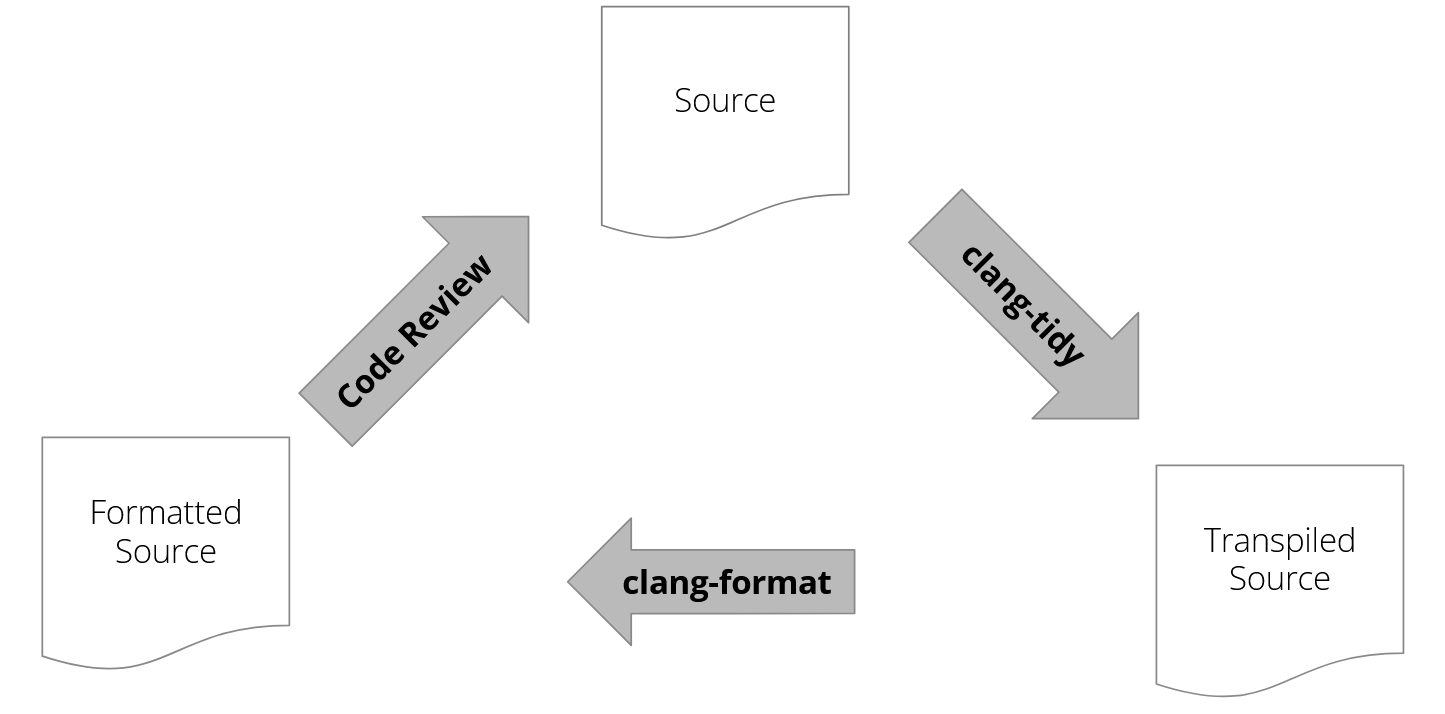
\includegraphics[width=1\textwidth]{source/Pictures/Screenshot 2025-04-25 122441.png}
        \caption{Steps involved in transforming code with clang-tidy}
        \label{figure:clang-tidy}
\end{figure}

\section{Limitations}

Although the design outlined in this chapter is feasible and satisfies our requirements, there are some limitations with this approach that should be addressed.

The largest issue is a limitation imposed by the C23 checked arithmetic headers: rewrites cannot be performed on all operations that could result in overflow. This is either due to type restrictions or the operations themselves. Approaches for how these limitations can be overcome are discussed in Chapter \ref{sec:conclusion}.

This approach is also specific to the LLVM family of compiler infrastructure, which means this approach will not work for codebases that require other compilers. Clang-tidy can technically work with C files meant for other compilers even if clang itself is unable to compiler them. The issue is the type information collected from the AST could error under certain circumstances, rendering the check ineffective. This issue is out of the scope of this project, however solving this design issue would catapult the effectiveness of such a tool.

It was mentioned that lines can be omitted from any changes from a clang-tidy check via the \texttt{//NOLINT} directive, however this will prevent changes to the entire line when a developer may want only a single expression to be omitted. This is not a major issue, however this could be a point for improvement in future work.

According to the Clang documentation, the AST matcher interface is not stable and is subject to change \cite{clang-interfaces}. Although this is a research endeavor and not a commercial project meant to have a long shelf life, this could be a deal breaker for a longer running project.

Finally, this approach will inherit the issue of difficult to read translations due to the automated nature of the tool. This is an unavoidable problem when designing an automated tool, however some ideas are also presented in Chapter \ref{sec:conclusion}.